\documentclass[dvipsnames]{article}

\usepackage{amsthm}
\usepackage{amsmath}
\usepackage{multicol}
\usepackage{amssymb}
\usepackage{mathabx}
\usepackage{accents}
\usepackage[english]{babel}
\usepackage{blindtext}
\usepackage{graphicx}
\usepackage{multicol}

\usepackage{tikz}
\usepackage{tkz-berge}
\usepackage{tkz-graph}

\usetikzlibrary{patterns,arrows,decorations.pathreplacing}

\usepackage{xcolor}
\definecolor{dblue}{RGB}{20,66,129}
\definecolor{rose}{RGB}{255,101,122}
\definecolor{crimsonred}{RGB}{132,22,23}
\definecolor{darkblue}{RGB}{72,61,139}

\definecolor{deepblue}{RGB}{36,123,160}
\definecolor{deepred}{RGB}{255,22,84}
\definecolor{deeporange}{RGB}{240,111,62}

\definecolor{olive}{rgb}{0.3, 0.4, .1}
\definecolor{fore}{RGB}{249,242,215}
\definecolor{back}{RGB}{51,51,51}
\definecolor{title}{RGB}{255,0,90}
\definecolor{dgreen}{rgb}{0.,0.6,0.}
\definecolor{gold}{rgb}{1.,0.84,0.}
\definecolor{JungleGreen}{cmyk}{0.99,0,0.52,0}
\definecolor{BlueGreen}{cmyk}{0.85,0,0.33,0}
\definecolor{RawSienna}{cmyk}{0,0.72,1,0.45}
\definecolor{Magenta}{cmyk}{0,1,0,0}





\theoremstyle{plain}
\newtheorem{lemma}{Lemma}
\newtheorem{prop}{Proposition}
\newtheorem*{example}{Example}
\newtheorem*{fact}{Fact}
\newtheorem{corollary}{Corollary}

\usepackage{algorithm}
\usepackage[noend]{algpseudocode}

\theoremstyle{plain}
\newtheorem{theorem}{Theorem}
\newtheorem{proposition}[theorem]{Proposition}
\newtheorem*{remark}{Remark}

\def\changemargin#1#2{\list{}{\rightmargin#2\leftmargin#1}\item[]}
\let\endchangemargin=\endlist 

\DeclareMathOperator{\codim}{codim}
\DeclareMathOperator{\lhdim}{\underline{\dim}_{\mathbf{M}}}
\DeclareMathOperator{\lmbdim}{\underline{\dim}_{\mathbf{MB}}}
\DeclareMathOperator{\biggercup}{\mathbin{\bigcup}}%

\title{Cartesian Products Avoiding Patterns}

\author{Jacob Denson\\ \and Malabika Pramanik\\ \and Joshua Zahl}

\begin{document}

\maketitle










\begin{abstract}
	We construct subsets of $[0,1]^d$ with large Hausdorff dimension whose Cartesian product avoids countably many sets with low Minkowski dimension. This generalizes the pattern avoidance problem often used in the literature. We use the result to construct high dimensional sets whose sum set avoids a given set, as well as construct dimension $1/2$ sets avoiding isosceles triangles, which are restricted to lie on an arbitrary set with fractional dimension close to that of a line. General pattern avoidance methods in the literature are completely unable to perform anything of this sort, which makes the latter result particularly surprising.
\end{abstract}










Can we construct high dimensional subsets of $\mathbf{R}^d$ avoiding patterns? For instance, can we find large sets containing no colinear triple of points? What about a set not containing any three vertices forming an isosceles triangle? If we can specify the pattern as the zero set of a function $f: (\mathbf{R}^d)^n \to \mathbf{R}$, results in the literature give general methods for finding sets $X \subset \mathbf{R}^d$ with large Hausdorff dimension such that for any distinct points $x_1, \dots, x_n \in X$, $f(x_1, \dots, x_n) \neq 0$. \cite{MalabikaRob} gives good results when $f$ is $C^1$ and $n$ is small, and \cite{Mathe} is successful when $f$ is a low degree polynomial. Rather than avoiding the zeroes of a function, in this paper, we fix a set $Z \subset (\mathbf{R}^d)^n$, and construct sets $X$ such that for any distinct $x_1, \dots, x_n \in X$, $(x_1, \dots, x_n) \not \in Z$. Surprisingly, a fractional dimension bound on $Z$ is all that is needed to find a high dimensional set $X$ in this setting.

\begin{theorem}
	Suppose $Z \subset (\mathbf{R}^d)^n$ is the countable union of compact sets, each with lower Minkowski dimension at most $\alpha$. Then there exists $X \subset [0,1]^d$ with
	%
	\[ \dim_{\mathbf{H}}(X) = \min \left( \frac{nd - \alpha}{n-1}, d \right) \]
	%
	such that if $x_1, \dots, x_n \in X$ are distinct, then $(x_1, \dots, x_n) \not \in Z$.
\end{theorem}

Our novel formulation of the pattern avoidance problem makes certain geometric features of $Z$ much more explicit than when we can  express $Z$ as the zero set of the function. In particular, exploiting the fractional dimension of $Z$ is completely non-obvious from the functional perspective. Moreover, the relation of the hypothesis of previous results to their conclusion when viewed as statements about the geometric set $Z$.

Despite the generality of our method, we are still able to recover Theorems 1.1 and 1.2 of \cite{MalabikaRob} as special cases when $Z$ is formed from a countable collection of smooth manifolds. Meanwhile, our proof is less technical than their approach. We compare our methods with \cite{MalabikaRob}, as well as other generic pattern avoidance methods, in Section 6.

Because our result if the only general avoidance method which can avoid singular sets $Z$, our method can be used to consider problems that other methods cannot touch at all. Most interesting of these results is a construction of a large `restricted' set avoiding configurations. In the restricted scenario, in addition to $Z$, we are given an arbitrary set $Y$, and we must construct a high dimensional $X$ avoiding $Z$ which is {\it restricted} to be a subset of $Y$. If $Y$ has non-empty interior, and $Z$ is smooth, we can apply the results of \cite{MalabikaRob} and \cite{Mathe} in this setting. But our result even applies for certain $Y$ with non-empty interior, or even a totally disconnected Cantor-like set. We discuss the applications of our method in Section 5.

The key idea to avoiding low dimension configurations is a random mass selection strategy. This is the main technique we use to approach a discrete variant of Theorem 1 in Section 2. The size of an optimal solution to the discrete problem is tricky to calculate exactly, but we can compute the expected size of a random selection, which is optimal enough in expectation, and is likely tight for general inputs to the problem. By overlaying the solution to the discretized problem at a sequence of scales, in Section 3 we are able to obtain the required set $X$ via a Cantor-type construction.

An important property of our discrete strategy is that it assigns mass `uniformly' at each iteration. Exploiting this fact, in Section 4 we are able to show the set $X$ has the required Hausdorff dimension regardless of how fast our sequence of scales decay. The uniform mass assignment technique occurs implicitly in at least one other Hausdorff dimension calculation, for example, in \cite{MalabikaRob}. But we do not believe the uniform strategy has been explicitly identified in the literature as a method to maintain fractional dimension despite a rapid decay of scales used in the construction of a set.

\begin{remark}
	The difficult setting of Theorem 1 occurs when $\alpha \geq d$. If $\alpha < d$,
	%
	\[ X = \left\{ x \in [0,1]^d : x \neq z_k\ \text{for all}\ (z_1, \dots, z_n) \in Z\ \text{and $1 \leq k \leq d$} \right\} \]
	%
	gives a set with full Hausdorff dimension satisfying the properties of the theorem. In our proof, we will assume $d \leq \alpha < dn$, and so must find a set $X$ with $\dim_{\mathbf{H}}(X) = (dn - \alpha) / (n-1)$.
\end{remark}









\section{Frequently Used Notation and Terminology}

Our argument heavily depends upon discretizing sets into unions of cubes. Throughout our argument, we use the following notation:

\begin{enumerate}
	\item[(A)] A {\it dyadic scale} is a length $l$ equal to $2^{-k}$ for some non-negative integer $k$.

	\item[(B)] Given a length $l$, $\mathcal{B}^d_l$ denotes the family of all half open cubes in $\mathbf{R}^d$ with side length $l$ and corners on the lattice $(l \cdot \mathbf{Z})^d$. That is,
	%
	\[ \mathcal{B}^d_l = \{ [a_1,a_1 + l) \times \dots \times [a_d, a_d + l) : a_i \in l \cdot \mathbf{Z} \}. \]
	%
	If $E \subset \mathbf{R}^d$, $\mathcal{B}^d_l(E)$ is the family of cubes in $\mathcal{B}^d_l$ intersecting $E$, i.e.
	%
	\[\mathcal{B}^d_l(E) = \{ I \in \mathcal{B}^d_l: I \cap E \neq \emptyset \}. \]
\end{enumerate}

In section 2, we solve a discrete version of our Theorem 1. Important to this approach is a discretization of the diagonal:

\begin{enumerate}
	\item[(C)] Given $I \in \mathcal{B}^{dn}_l$, we can decompose $I$ as $I_1 \times \dots \times I_n$ for unique cubes $I_1, \dots, I_n \in \mathcal{B}^d_l$. We say $I$ is {\it weakly non-diagonal} if the cubes $I_1, \dots, I_n$ are distinct. 
\end{enumerate}

In section 3, we discretize the set $Z$ in the hypothesis of Theorem 1 into a union of boxes in order to construct our solution $X$. Our argument is aided by the following definitions:

\begin{enumerate}
	\item[(D)] Adopting the terminology of \cite{KatzTao}, we say a collection of sets $U_1, U_2, \dots$ is a {\it strong cover} of some set $E$ if $E \subset \limsup U_k$, which means every element of $E$ is contained in infinitely many of the sets $U_k$.

	\item[(E)] The {\it lower Minkowski dimension} of a compact set $Z \subset \mathbf{R}^d$ is
	%
	\begin{equation} \label{lowerminkdim}
		\lhdim(Z) = \liminf_{l \to 0} \frac{\log( \#( \mathcal{B}^d_l(Z) ) )}{\log(1/l)}.
	\end{equation}
	%
	This means if $\mathcal{B}^d_l(E) \leq \alpha$, there is a sequence of lengths $l_1, l_2, \to 0$ and positive $\delta_1, \delta_2, \dots \to 0$ such that $\#(\mathcal{B}^d_{l_k}(Z)) \leq (1/l_k)^{\alpha + \delta_k}$.
\end{enumerate}

Once $X$ has been constructed, in Section 4 we show that it has the Hausdorff dimension guaranteed by Theorem 1. Here we use a Frostman's lemma type approach, summarized by the following definitions:

\begin{enumerate}
	\item[(F)] The $\alpha$ dimensional Hausdorff measure $H^\alpha$ on $\mathbf{R}^d$ is defined to be $H^\alpha(E) = \lim_{\delta \to 0} H^\alpha_\delta(E)$, where
	%
	\begin{equation} \label{hausdorffdef}
		H^\alpha_\delta(E) = \inf \left\{ \sum_{k = 1}^m l_k^\alpha : E \subset \bigcup_{k = 1}^m I_k, \begin{array}{c} \text{each}\ I_k\ \text{is a dyadic cube}\\
		\text{of length $l_k \leq \delta$} \end{array} \right\}.
	\end{equation}
	%
	The {\it Hausdorff dimension} of a set $E$ is
	%
	\[ \dim_{\mathbf{H}}(E) = \inf \{ \alpha \geq 0 : H^\alpha(E) = 0 \} \]


	\item[(G)] A {\it Frostman measure} of dimension $\alpha$ is a non-zero compactly supported finite Borel measure $\mu$ on $\mathbf{R}^d$ such that for any dyadic scale $l$, and $I \in \mathcal{B}^d_l$, $\mu(I) \lesssim l^\alpha$. {\it Frostman's lemma} shows that
	%
	\begin{equation} \label{frostmandef}
		\dim_{\mathbf{H}}(E) = \sup \left\{ \alpha: \begin{array}{c} \text{there is an}\ \alpha\ \text{dimensional Frostman}\\
	\text{measure supported on $E$} \end{array} \right\},
	\end{equation}
\end{enumerate}










\section{Avoidance at Discrete Scales}

We avoid $Z$ via a multi-scale construction at an infinite sequence of scales. At each scale, we solve a discretized version of the problem. Combining these solutions then solves the original problem. This section describes the discretized avoidance technique. This is the {\it core} part of our construction, and the Hausdorff dimension we achieve is a direct result of our success in the discrete setting.

Fix two dyadic scales $l$ and $s$, with $l > s$. In the discrete setting, we replace $Z$ by a union of side length $s$ cubes in $\mathbf{R}^{dn}$, denoted $Z_D$. Our goal is to take a set $E$, which is a union of side length $l$ cubes, and find a union of side length $s$ cubes $F \subset E$ such that $F^n$ is disjoint from the weakly non-diagonal (see definition C) subcubes of $Z_D$.

In order to ensure that $X$ has large Hausdorff dimension, it is crucial that the mass of $F$ is spread uniformly over $E$ in the discrete setting. We can achieve this by trying to include a equal portion of mass in each side length $r$ sub cube of $E$, for some intermediary dyadic scale $r$ between $l$ and $s$. The next lemma shows that we can select a equal portion of mass from {\it almost} all the side length $r$ cubes, provided that $|Z_D| \ll |E| r^{d(n-1)}$.

\begin{figure}
	\centering
    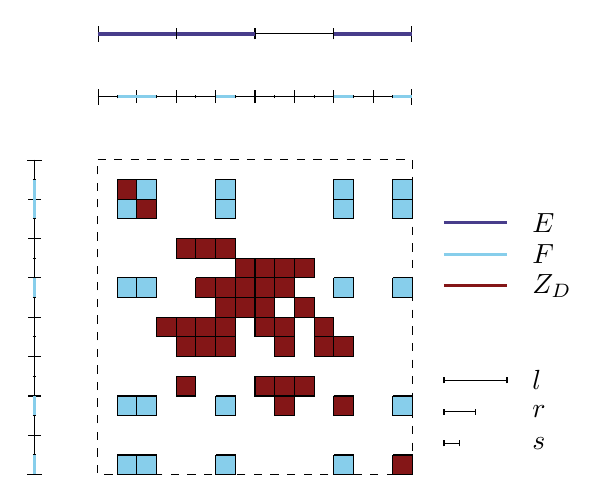
\begin{tikzpicture}[scale=4] %% Change scaling as needed
        \draw [|-]  (0,0) -- (1/4,0);
		\draw (0,0) -- (1,0);
        \draw [-|] (3/4,0) -- (1,0);% node [anchor = south west] {$E$};

        \foreach \x in {1,2,3}
        	\draw (\x/4,-0.5pt) -- (\x/4,0.5pt);

        \foreach \x in {0,1,3}
    		\draw[darkblue, ultra thick] (\x/4+0.001,0) -- (\x/4 + 1/4-0.001,0);




        \draw [|-]  (0,-0.2) -- (1/4,-0.2);
        \draw (0,-0.2) -- (1,-0.2);
        \draw [-|] (6/7,-0.2) -- (1,-0.2);% node [anchor = north west] {$F$};

        \foreach \x in {1,...,15}
            \draw (\x/16,-0.2-0.005) -- (\x/16,-0.2+0.005);

        \foreach \x in {1,...,7}
            \draw (\x/8,-0.2-0.02) -- (\x/8,-0.2+0.02);

        \foreach \x in {1,2,6,12,15}
            \draw[SkyBlue, very thick] (\x/16+0.001,-0.2) -- (\x/16 + 1/16 - 0.001,-0.2);








        \draw [|-]  (-0.2,-0.4) -- ++(0,-0.01);
        \draw (-0.2,-0.4) -- (-0.2,-1.4);
        \draw [-|] (-0.2,-1.38) -- (-0.2,-1.4);% node [anchor = north east] {$F$};

        \foreach \x in {1,...,15}
            \draw (-0.2-0.005,-0.4-\x/16) -- (-0.2+0.005,-0.4 -\x/16);

        \foreach \x in {1,...,7}
            \draw (-0.2-0.02,-0.4-\x/8) -- (-0.2+0.02,-0.4-\x/8);

        \foreach \x in {1,2,6,12,15}
        	\draw[SkyBlue, very thick] (-0.2,-0.4-\x/16-0.001) -- (-0.2,-0.4-\x/16-1/16+0.001);





        \draw[dashed] (0,-0.4) -- (1,-0.4) -- (1,-1.4) -- (0,-1.4) -- (0,-0.4);

        \foreach \x in {1,2,6,12,15}
        	\foreach \y in {1,2,6,12,15}
        		\draw[fill=SkyBlue] (\x/16,-0.4 - \y/16) -- ++(0,-1/16) -- ++ (1/16,0) -- ++(0,1/16) -- ++(-1/16,0);

        \foreach \x in {1,2,6,12,15}
        	\draw[fill=crimsonred] (\x/16,-0.4 - \x/16) -- ++(0,-1/16) -- ++ (1/16,0) -- ++(0,1/16) -- ++(-1/16,0);

        \foreach \x/\y in {4/4, 5/4, 6/4, 7/5, 8/5, 9/5, 10/5, 5/6, 6/6,7/6,8/6,9/6, 6/7, 7/7, 8/7, 10/7, 3/8, 4/8, 5/8, 6/8, 8/8, 9/8, 11/8, 4/9, 5/9, 6/9, 9/9, 11/9, 12/9, 4/11, 8/11, 9/11, 10/11, 9/12}
        	\draw[fill=crimsonred] (\x/16,-0.4 - \y/16) -- ++(0,-1/16) -- ++ (1/16,0) -- ++(0,1/16) -- ++(-1/16,0);







            \draw [darkblue, very thick] (1.1,-0.6) -- (1.3,-0.6);
%            \foreach \x in {1.1, 1.3}
%                \draw (\x,-0.6 - 0.01) -- (\x,-0.6 + 0.01);
            \draw (1.35,-0.6) node [anchor = west] {$E$};

            \draw [SkyBlue, very thick] (1.1,-0.7) -- (1.3,-0.7);
%            \foreach \x in {1.1,1.3}
%                \draw (\x,-0.7 - 0.01) -- (\x, -0.7 + 0.01);
            \draw (1.35,-0.7) node [anchor = west] {$F$};

            \draw [crimsonred, very thick] (1.1,-0.8) -- (1.3,-0.8);
%            \foreach \x in {1.1,1.3}
%                \draw (\x,-0.8 - 0.01) -- (\x, -0.8 + 0.01);
            \draw (1.35,-0.8) node [anchor = west] {$Z_D$};

            \draw (1.1,-1.1) -- (1.3,-1.1);
            \foreach \x in {1.1, 1.3}
                \draw (\x,-1.1 - 0.01) -- (\x,-1.1 + 0.01);
            \draw (1.35,-1.1) node [anchor = west] {$l$};

            \draw (1.1,-1.2) -- (1.2,-1.2);
            \foreach \x in {1.1, 1.2}
                \draw (\x,-1.2 - 0.01) -- (\x,-1.2 + 0.01);
            \draw (1.35,-1.2) node [anchor = west] {$r$};

            \draw (1.1,-1.3) -- (1.15,-1.3);
            \foreach \x in {1.1, 1.15}
                \draw (\x,-1.3 - 0.01) -- (\x,-1.3 + 0.01);
            \draw (1.35,-1.3) node [anchor = west] {$s$};
	\end{tikzpicture}
	\caption{An example choice of $F$ satisfying the conclusions of Lemma 1 where $d = 1$ and $n = 2$. $F$ satisfies the non-concentration and avoidance property, as well as containing an interval from all but 3 of the intervals in $\mathcal{B}^d_r(E)$.}
\end{figure}
%TODO: Make figure into two-or three distinct figures indicating the process.

\begin{lemma}
	Fix three dyadic lengths $l > r > s$. Let $E$ be a union of cubes in $\mathcal{B}^d_l$, and $Z_D$ a union of cubes in $\mathcal{B}^{dn}_s$. Then there exists $F \subset E$, which is a union of cubes in $\mathcal{B}^d_s$, such that
	%
	\begin{itemize}
		\item \emph{Avoidance}:  For any distinct $I_1, \dots, I_n \in \mathcal{B}^d_s(F)$, $I_1 \times \dots \times I_n \not \in \mathcal{B}^{dn}_s(Z_D)$.
		\item \emph{Non-Concentration}: $F$ contains at most one sidelength $s$ subcube of each cube in $\mathcal{B}^d_r(E)$.
		\item \emph{Breadth}: For all but $|Z_D| r^{-dn}$ of the cubes in $\mathcal{B}^d_r(E)$, $F$ contains a sidelength $s$ subcube.
	\end{itemize}
\end{lemma}
\begin{proof}
	Form a random set $U$ by selecting a side length $s$ cube from each side length $r$ cube uniformly at random. More precisely, set
	%
	\[ U = \bigcup\; \{ J_I: I \in \mathcal{B}^d_r(E) \}, \]
	%
	where $J_I$ is an element selected uniformly randomly from $\mathcal{B}^d_s(I)$. Then $U$ certainly satisfies the non-concentration and breadth properties, but $U$ does not satisfy the avoidance property. We will show that with non-zero probability, we can obtain the avoidance property by removing at most $|Z_D|r^{-dn}$ cubes from $U$, so that the breadth property remains satisfied.

	For any $J \in \mathcal{B}^d_s(E)$, there is a unique $I \in \mathcal{B}^d_r(E)$ such that $J \subset I$, so
	%
	\[ \mathbf{P}(J \subset U) = \mathbf{P}(J_I = J) = (s/r)^d. \]
	%
	Since any two elements of $\mathcal{B}^d_s(U)$ lie in distinct cubes of $\mathcal{B}^d_r$, the only way that a {\it weakly non-diagonal} cube $K = J_1 \times \dots \times J_n$ in $\mathcal{B}^{dn}_s(Z_D)$ is a subset of $U^n$ is if $J_1, \dots J_n$ all lie in separate cubes of $\mathcal{B}^d_r$. In this case, the events $\{ J_k \subset U \}$ are independent of one another, and so
	%
	\begin{align*}
		\mathbf{P}(K \subset U^n) &= \mathbf{P}(J_1 \subset U) \cdots \mathbf{P}(J_n \subset U) = (s/r)^{dn}.
	\end{align*}
	%
	If $\mathcal{K}(U)$ denotes the family of all weakly non-diagonal cubes $K \in \mathcal{B}^{dn}_s(Z_D)$ contained in $U^n$, then, letting $K$ range over the weakly non-diagonal cubes of $\mathcal{B}^{dn}_s(Z_D)$, we find
	%
	\begin{align*}
		\mathbf{E}(\# (\mathcal{K}(U))) &= {\sum}_K\; \mathbf{P}(K \subset U^n) \leq |\mathcal{B}^{dn}_s(Z_D)| (s/r)^{dn} = |Z_D| r^{-dn}.
	\end{align*}
	%
	In particular, there is at least one outcome $U_0$ for $U$ we can choose for which
	%
	\[ \#(\mathcal{K}(U_0)) \leq \mathbf{E}(\mathcal{K}(U)) = |\mathcal{B}^{dn}_s(Z_D)| (s/r)^{dn} = |Z_D| r^{-dn}. \]
	%
	Thus we have selected a section of mass with very few intersections with $Z_0$.

	We now define $F = U_0 - \{ J_1 : K = J_1 \times \dots \times J_n \in \mathcal{K}(U_0) \}$. As a subset of $U_0$, $F$ inherits the non-concentration property. We have removed at most $|Z_D| r^{-dn}$ cubes from $U_0$, so $F$ satisfies the breadth property. Finally, since we have removed a single side from every weakly non-diagonal cube in $U_0^n$ intersecting $Z_D$, $F$ satisfies the avoidance property. So our construction is complete.
\end{proof}

\begin{remark}
	The existence of $U_0$ was justified by a randomized selection process. Nonetheless, its existence can be made constructive: We simply iterate through all possible outcomes of $U$ and pick one minimizing the cardinality of $\mathcal{K}(U)$. As a result, the set $X$ in our theorem is obtained by explicit, constructive means.
\end{remark}

If the set $Z$ has dimension $\alpha$, we will later show its discretization $Z_D$ will satisfy bounds of the form $|Z_D| \leq s^{dn-\gamma}$, with $\gamma$ converging to $\alpha$ as $s \to 0$. For convenience, we will also set $r$ to be the closest dyadic scale to $s^\lambda$, for some $\lambda \in (0,1)$. The size of $\lambda$ is directly related to the Hausdorff dimension of the set $X$ we construct, are the next corollary shows precisely how large we can set it to be so that $F$ contains subcubes from a constant fraction of the cubes in $\mathcal{B}^d_r(E)$. The error term $3m \log_s |E|$ will be made insignificant by the rapid decay of the values $s$ used in our construction.

\begin{corollary}
	Fix two dyadic scales $l > r$. Let $E$ be a union of cubes in $\mathcal{B}^d_l$, and $Z_D$ a union of cubes in $\mathcal{B}^{dn}_s$. Also, consider three parameters $\lambda \in (0,1]$, $\gamma \in [d,dn)$, and $m > 0$. Suppose $r$ is the closest dyadic scale to $s^\lambda$, i.e. $r = 2^{- \lfloor \lambda \log_2(1/s) \rfloor}$, $|E| \leq 1/2$, and $|Z_D| \leq s^{dn-\gamma}$. If
	%
	\begin{equation} \label{corollaryinequality}
		0 < \lambda \leq \frac{dn - \gamma}{d(n-1)} - 3 m \log_s |E|,
	\end{equation}
	%
	then we can find $F$ satisfying the avoidance, and non-concentration property, containing intervals from all but a fraction $1/2^m$ of the cubes in $\mathcal{B}^d_r(E)$.
\end{corollary}
\begin{proof}
	Rearranging (\ref{corollaryinequality}) gives
	%
	\begin{align*}
		dn - \gamma - \lambda d(n-1) &\geq 3d(n-1) m \log_s |E|.
	\end{align*}
	%
	Since $r$ is within a factor of two from $s^\lambda$, we consider the set $E$ obtained from Lemma 1, and we calculate that
	%
	\begin{align*}
		&\frac{|\{ I \in \mathcal{B}^d_r(E): \mathcal{B}^d_s(I) \cap \mathcal{B}^d_s(F) = \emptyset \}|}{|\mathcal{B}^d_r(E)|} \leq \frac{|Z_D| r^{-dn}}{|E|r^{-d}} \leq \frac{s^{dn - \gamma} r^{-dn}}{|E| r^{-d}}\\
		&\ \ \ \ \ \leq s^{dn - \gamma} r^{-d(n-1)} |E|^{-1} \leq (s^{dn - \gamma}) (s/2)^{- \lambda d(n-1)} |E|^{-1}\\
		&\ \ \ \ \ \leq 2^{\lambda d(n-1)} s^{dn - \gamma - \lambda d(n-1)} |E|^{-1} \leq 2^{\lambda d(n-1)} |E|^{3d(n-1)m - 1}\\
		&\ \ \ \ \ \leq 2^{d(n-1) - (3d(n-1)m - 1)} \leq 1/2^m.
	\end{align*}
	%
	The final inequality is true because
	%
	\[ [d(n-1) - (3d(n-1)m - 1)] =  1 - d(n-1)(3m - 1) \leq 1 - 2m \leq -m. \tag*{\qedhere} \]
\end{proof}

\begin{remark}
	We reemphasize that the discrete method is the core of our avoidance technique. The remaining argument is modular. Indeed, we based the remaining parts of our paper on the construction method of \cite{MalabikaRob}. If for a special case of $Z$, one can improve the lemma so that fewer cubes are discarded, then the remaining parts of our paper can likely be applied near verbatim to yield a set $X$ with a larger Hausdorff dimension. For instance, if $Z$ is a degree $m$ algebraic hypersurface, and $Z_D = \mathcal{B}^{dn}_l(Z)$, then a variation on the technique used in Proposition 2.2 of \cite{Mathe} enables one to obtain a version of Corollary 1 with $\lambda \approx 1/m$. Following through the remainder of our proof replicates Theorem 2.3 of \cite{Mathe}.
\end{remark}










\section{Fractal Discretization}

Now we apply the discrete result at many scales. The fact that $Z$ is the countable union of compact sets with Minkowski dimension $\alpha$ implies that we can find an efficient {\it strong cover} (see definition D) of $Z$ by cubes restricted to lie at a sequence of dyadic scales $l_k$ converging to zero arbitrarily fast.

\begin{lemma}
	Let $Z \subset \mathbf{R}^{dn}$ be a countable union of compact sets, each with lower Minkowski dimension at most $\alpha$, and consider any decreasing sequence $\varepsilon_k$ converging to zero with $\alpha + \varepsilon_k \leq dn$. Then there is a decreasing sequence of dyadic scales $l_1, l_2, \dots$, and compact sets $Z_k$, which is a union of cubes in $\mathcal{B}^{dn}_{l_k}$, such that $Z$ is strongly covered by the sets $Z_k$ and $\#( \mathcal{B}^{dn}_{l_k}(Z_k) ) \leq 1/l_k^{\alpha + \varepsilon_k}$.
\end{lemma}
\begin{proof}
	Let $Z$ be the union of sets $Y_i$ with $\lhdim(Y_i) \leq \alpha$ for each $i$. Consider any sequence of integers $m_1, m_2, \dots$which repeats each integer infinitely often. Given $k$, since $\lhdim(Y_{m_k}) \leq \alpha$, equation (\ref{lowerminkdim}) implies there are infinitely many lengths $l$ with $\#(\mathcal{B}^{dn}_l(Y_{m_k})) \leq 1/l^{\alpha + (\varepsilon_k/2)}$. Replacing $l$ with a dyadic number at most twice the size of $l$, there are infinitely many {\it dyadic} lengths $l$ with
	%
	\[ \# (\mathcal{B}^{dn}_l(Y_{m_k})) \leq 1/(l/2)^{\alpha + \varepsilon_k} \leq 2^{dn}/l^{\alpha + (\varepsilon_k/2)} = (2^{dn} l^{(\varepsilon_k/2)}) / l^{\alpha + \varepsilon_k} . \]
	%
	In particular, we may fix a length $l_k$ smaller than $l_1, \dots, l_{k-1}$, which in addition satisfies the inequality $2^{dn} l^{(\varepsilon_k/2)} \leq 1$ so that $\# ( \mathcal{B}^{dn}_l(Y_{m_k})) \leq 1/l^{\alpha + \varepsilon_k}$. Then the union of the cubes in $\mathcal{B}^{dn}_{l_k}(Y_{m_k})$ forms the set $Z_k$.
\end{proof}

\begin{remark}
	In the proof, we are free to make $l_k$ arbitrarily small in relation to the previous parameters $l_1, \dots, l_{k-1}$ we have chosen. For instance, in Section 4, we will assume that $l_{k+1} \leq l_k^{k^2}$, and the argument above can be easily modified to incorporate this inequality. We will also find that setting $\varepsilon_k = c \cdot k^{-1}$ suffices to give the results we need, where $c$ is a sufficiently small constant such that $\alpha + c \leq dn$.
\end{remark}

We can now construct $X$ by avoiding the various discretizations of $Z$ at each scale. The aim is to find a nested decreasing family of discretized sets $X_k$ with $X = \lim X_k$. One condition guaranteeing that $X$ avoids $Z$ is that $X_k^n$ is disjoint from {\it weakly non-diagonal} cubes (see definition D) in $Z_k$.

\begin{lemma}
	Suppose $Z_k$ is a strong cover of $Z$, where $Z_k$ is a union of cubes in $\mathcal{B}^{dn}_{l_k}$ with $l_k \to 0$, and $X_k$ is a nested decreasing family of sets such that for each $k$, $X_k^n$ is disjoint from weakly non-diagonal cubes in $Z_k$. If $X = \lim X_k$, then $(x_1, \dots, x_n) \not \in Z$ for any distinct $x_1, \dots, x_n \in X$.
\end{lemma}
\begin{proof}
	Pick $z \in Z$ with distinct coordinates $z_1, \dots, z_n$. Set
	%
	\[ \Delta = \{ w \in (\mathbf{R}^d)^n : \text{there exists}\ i \neq j\ \text{such that}\ w_i = w_j \}. \]
	%
	Then $d(\Delta,z) > 0$, where $d$ is the Hausdorff distance. Since $Z_k$ is a strong cover of $Z$, the point $z$ is covered by cubes in infinitely many of collections $Z_{k_m}$. For suitably large $m$, the sidelength $l_k$ cube $I$ in $Z_{k_m}$ containing $z$ is disjoint from $\Delta$. But this means that $I$ is weakly non-diagonal, and so $z \not \in X_m^d$. In particular, $z$ is not an element of $X^n$.
\end{proof}

We now quite simply iterate our discrete scale argument to construct the set $X$. First, we set $X_0 = [0,1/2]^d$, so that $|X_0| \leq 1/2$, enabling us to apply Corollary 1. To get $X_{k+1}$ from $X_k$, we apply Corollary 1, setting $E = X_k$, $Z_D = Z_{k+1}$, $l = l_k$, $s = l_{k+1}$, $\gamma = \alpha + \varepsilon_k = \alpha + c \cdot k^{-1}$, and $r$ the closest dyadic scale to $l_{k+1}^{\beta_{k+1}}$, where
%
\begin{equation} \label{betadef}
	\beta_{k+1} = \frac{dn - \alpha}{d(n-1)} - \left( \frac{\varepsilon_{k+1}}{d(n-1)} + 6(k+1) \log_{L_{k+1}} |X_k| \right).
\end{equation}
%
We can now apply Corollary 1 to constructs a set $F$ with $F^n$ avoiding weakly non-diagonal cubes in $Z_{k+1}$, and containing a $\mathcal{B}^d_{l_{k+1}}$ subcube from all but a fraction $1/2^{2k +2}$ of the $\mathcal{B}^d_{r_{k+1}}$ cubes in $I$. We set $X_{k+1} = F$. Repeatedly doing this builds an infinite sequence of the $X_k$. Since $X_k^n$ avoids $Z_k$, for any distinct $x_1, \dots, x_n \in X$, $(x_1, \dots, x_n) \not \in X$.










\section{Dimension Bounds}

All that remains in our argument is showing $X$ has the right Hausdorff dimension. First, we begin with a rough outline of our proof strategy. At the discrete scale $l_k$, $X$ looks like a $d \beta_k$ dimensional set. If the lengths $l_k$ rapidly converge to zero, then we can ensure $\beta_k \to \beta$, where
%
\[ \beta = \frac{dn - \alpha}{d(n - 1)}. \]
%
Thus $X$ looks $d \beta = (dn - \alpha) / (n-1)$ dimensional at the discrete scales $l_k$, which is the Hausdorff dimension we want. To obtain the complete dimension bound, it then suffices to interpolate to get a $d\beta$ dimensional behavior at all intermediary scales. We won't be penalized here by making the gaps between discrete scales too large, because the uniform way that we have selected cubes in consecutive scales implies that between the scales $l_k$ and $l_{k+1}^\beta$, $X$ behaves like a full dimensional set. This is the uniform mass assignment technique mentioned in the introduction.

\begin{lemma}
	$\beta_k = \beta - O(1/k)$.
\end{lemma}
\begin{proof}
	We must show
	%
	\[ \beta - \beta_k = \frac{\varepsilon_{k+1}}{d(n-1)} + 6(k+1) \log_{l_{k+1}} |X_k| = O(1/k). \]
	%
	Since $\varepsilon_k = c \cdot k^{-1}$, the first term is easily seen to be $O(1/k)$. On the other hand, we need the lengths to tend to zero rapidly to make the other error term decay to zero. The remark after Lemma 2 infers we can assume $l_{k+1} \leq l_k^{k^2}$, so we find
	%
	\[ (k+1) \log_{l_{k+1}} |X_k| \leq \frac{(k+1) \log l_k}{\log l_{k+1}} \leq \frac{(k+1) \log l_k}{k^2 \log l_k} = \frac{k+1}{k^2} = O(1/k). \]
	%
	Thus both components of the error term are $O(1/k)$.
\end{proof}

The most convenient way to understand the dimension of $X$ at various scales is to use a Frostman type approach. We construct a finite Borel measure $\mu$ supported on $X$ which is a Frostman measure (see definition G) of dimension $d \beta - \varepsilon$ for each $\varepsilon > 0$. Combined with Frostman's lemma, this implies that $\dim_{\mathbf{H}}(X) \geq d \beta$. The advantage of this approach is that once a natural choice of $\mu$ is fixed, the behaviour of $X$ at a scale $l$ can be understood by looking at the behaviour of $\mu$ restricted to cubes at the scale $l$.

To construct $\mu$, we take a sequence of measures $\mu_k$, supported on $X_k$, and then take a weak limit. We initialize this construction by setting $\mu_0$ to be the uniform probability measure on $X_0 = [0,1/2]^d$. We then define $\mu_{k+1}$, supported on $X_{k+1}$, by modifying the distribution of $\mu_k$. First, we throw away the mass of the cubes in $\mathcal{B}^d_{l_k}(X_k)$ for which more than half of the cubes in $\mathcal{B}^d_{r_{k+1}}(I)$ are disjoint from $X_{k+1}$. For the cubes $I$ with more than half of the cubes $\mathcal{B}^d_{r_{k+1}}(I)$ containing a part of $X_{k+1}$, we distribute the mass $\mu_k(I)$ uniformly over the subcubes of $I$ in $X_{k+1}$, giving the distribution of $\mu_{k+1}$.

A glance at the cumulative distribution functions of the $\mu_k$ shows these measures converge weakly to a function $\mu$. For any $I \in \mathcal{B}^d_{l_k}$, we find $\mu(I) \leq \mu_k(I)$, which will be useful for passing from bounds on the discrete measures to bounds on the final measure.

\begin{lemma}
	If $I \in \mathcal{B}^d_{l_k}$, then
	%
	\begin{equation} \label{measurebound}
		\mu(I) \leq \mu_k(I) \leq 2^k \left[ \frac{r_k r_{k-1} \dots r_1}{l_{k-1} \dots l_1} \right]^d.
	\end{equation}
\end{lemma}
\begin{proof}
	Consider $J \in \mathcal{B}^d_{l_{k-1}}$ with $I \subset J$. If $\mu_k(I) > 0$, more than half of the elements of $\mathcal{B}^d_{r_k}(J)$ contain a single sidelength $l_k$ subcube in $X_k$. Since the mass $\mu_{k-1}(J)$ distributes itself evenly over all such cubes, of which there must be more than $2^{-1} (l_{k-1} / r_k)^d$, we find
	%
	\[ \mu_k(I) \leq 2(r_k/l_{k-1})^d \mu_{k-1}(J) \]
	%
	Expanding this inequality recursively completes the proof, using the fact that $\mu_0$ has total mass one as a base case.
\end{proof}

\begin{corollary}
	The measure $\mu$ is non-zero.
\end{corollary}
\begin{proof}
	The nonconcentration property at each discrete scales implies that for each $k$,
	%
	\[ \# (\mathcal{B}^d_{l_k}(X_k)) \leq \left[ \frac{l_{k-1} \dots l_1}{r_k \dots r_1} \right]^d. \]
	%
	Since only a fraction $1/2^{2k+2}$ of the cubes in $\mathcal{B}^d_{r_k}(X_k)$ do not contain an cube in $X_{k+1}$, it is only for at most a fraction $1/2^{2k+1}$ of the cubes in $\mathcal{B}^d_{r_k}(X_k)$ cubes that $X_{k+1}$ fails to contain more than half of the subcubes. But this means that
	%
	\[ \mu_k[0,1]^d - \mu_{k+1}[0,1]^d \leq \left( \frac{1}{2^{2k + 1}} \left[ \frac{l_{k-1} \dots l_1}{r_k \dots r_1} \right]^d \right) \left( 2^{k} \left[ \frac{r_k \dots r_1}{l_{k-1} \dots l_1} \right]^d \right) \leq 1/2^{k+1}. \]
	%
	Thus for any $m$,
	%
	\begin{align*}
		\mu_m [0,1]^d &= \mu_0 [0,1]^d - \left( \sum_{k = 0}^{m-1} \mu_k [0,1]^d - \mu_{k+1} [0,1]^d \right) \geq 1 - \sum_{k = 0}^{m-1} 1/2^{k+1} \geq 1/2.
	\end{align*}
	%
	Since $m$ was arbitrary, this implies $\mu [0,1]^d \geq 1/2$, so in particular, $\mu \neq 0$.
\end{proof}

Treating all parameters in equation (\ref{measurebound}) which depend on indices smaller than $k$ as essentially constant, we `conclude' that $\mu_k(I) \lesssim r_k^d \lesssim l_k^{\beta d - O(1/k)}$. The equation $l_{k+1} \leq l_k^{k^2}$ implies $l_k$ decays very rapidly, which enables us to rigorously obtain this inequality.

\begin{corollary}
	For all $I \in \mathcal{B}^d_{l_k}$, $\mu(I) \leq \mu_k(I) \lesssim l_k^{d \beta - O(1/k)}$.
\end{corollary}
\begin{proof}
	Given $\varepsilon > 0$, equation (\ref{measurebound}) and the inequality $l_k \leq l_{k-1}^{(k-1)^2}$ imply
	%
	\begin{align*}
		\mu_k(I) &\leq 2^k \left[ \frac{r_k \dots r_1}{l_{k-1} \dots l_1} \right]^d \leq \left( \frac{2^k}{l_{k-1}^d \dots l_1^d} \right) l_k^{d \beta_k}\\
		&\leq \left( 2^k l_k^{2d/k} / l_{k-1}^{d(k-1)} \right) l_k^{d \beta_k - 2d/k}\\
		&\leq \left( 2^k l_{k-1}^{(2d/k) (k-1)^2 - d(k - 1)} \right) l_k^{d \beta_k - 2d/k} = o(l_k^{d\beta_k - 2d/k}). \tag*{\qedhere}
	\end{align*}
\end{proof}

%It is intuitive that the mass on $\mu$ will distribute more thinly at each stage the fatter the cubes we keep on each iteration of the discrete scale argument. Quantifying this leads directly to our result. We will prove that for each length $L$ interval $I$, $\mu(I) \lesssim_N L^{\beta_N}$. Thus Frostman's lemma guarantees that $\dim_{\mathbf{H}}(X) \geq \beta_N$, and taking $\beta_N \to \beta$ will complete the proof.

%We now rely on a covering argument to show $X$ looks $d \beta$ dimensional at all the intermediary scales. Here we won't be penalized by the fact that the $L_k$ rapidly tend to zero, because the uniformity property implies $X$ looks {\it full} dimensional between the scales $L_k$ and $R_{k+1}$. We fix an increasing sequence $\beta_k'$ with $\beta_k' < \beta_k$, and $\beta_k' \to \beta$ as $k \to \infty$. This gives us slightly more room to bound mass when obtaining the Frostman's lemma result. We set $\beta_k' - \beta_k = 1/k$ to obtain the choice of $L_N$ given as an example.

%\begin{corollary}
%	If $L_k \ll 1$, $\mu(I) \leq L_k^{d \beta_k'}$ for $I \in \mathcal{B}(L_k)$.
%\end{corollary}
%\begin{proof}
%	We can rewrite the inequality in the last problem as
	%
%	\[ \mu(I) \leq \left[ 2^k \left( \frac{R_{k-1} \dots R_1}{L_{k-1} \dots L_1} \right)^d R_k^d L_k^{- d \beta_k'} \right] L_k^{d\beta_k'} \]
	%
%	Now $R_k^d L_k^{-d\beta_k'} \leq (2L_k^{\beta_k})^d L_k^{-d\beta_k'} \leq 2^d L_k^{d(\beta_k - \beta_k')}$, which tends to zero as $L_k \to \infty$, while the remaining parameters are fixed. Thus if $L_k$ is sufficiently small, we can bound the constant in the square brackets by $1$, which is sufficient to obtain the inequality.
%\end{proof}

Corollary 3 gives the cleanest expression of the $d \beta$ dimensional behavior of $\mu$ at discrete scales we will need. To obtain a Frostman measure bound at {\it all} scales, we need to apply a covering argument. This is where the uniform mass assignment technique comes into play. Because $\mu$ behaves like a full dimensional Frostman measure between the discrete scales $r_{k+1}$ and $l_k$, the argument below shows the gap between $l_k$ and $r_{k+1}$ can be arbitrary. This is essential to our argument, because $l_k$ decays faster than $2^{-k^m}$ for any $m > 0$.

\begin{lemma}
	If $l \leq l_k$ is dyadic and $I \in \mathcal{B}^d_l$, then $\mu(I) \lesssim l^{d\beta - O(1/k)}$.
\end{lemma}
\begin{proof}
	We use a covering argument, which breaks into cases depending on the size of $l$ in proportion to $l_k$ and $r_k$:
	%
	\begin{itemize}
		\item If $r_{k+1} \leq l \leq l_k$, we can cover $I$ by $(l/r_{k+1})^d$ cubes in $\mathcal{B}^d_{r_{k+1}}$. Because of the non-concentration and breadth properties of our construction, we therefore know that the mass of each cube in $\mathcal{B}^d_{r_{k+1}}$ is bounded by at most $2(r_{k+1}/l_{k+1})^d$ times the mass of a $\mathcal{B}^d_{l_k}$ cube. Thus
		%
		\begin{align*}
			\mu(I) &\lesssim (l/r_{k+1})^d (2(r_{k+1}/l_k)^d) l_k^{d \beta - O(1/k)} \leq 2 l^d / l_k^{d + O(1/k) - d \beta} \leq 2 l^{d \beta - O(1/k)}.
		\end{align*}

		\item If $l_{k+1} \leq l \leq r_{k+1}$, we can cover $I$ by a single cube in $\mathcal{B}^d_{r_{k+1}}$. Each cube in $\mathcal{B}^d_{r_{k+1}}(X)$ contains at most one cube in $\mathcal{B}^d_{l_{k+1}}(X)$, so
		%
		\[ \mu(I) \lesssim l_{k+1}^{d\beta - O(1/k)} \leq l^{d \beta - O(1/k)}. \]

		\item If $l \leq l_{k+1}$, there certainly exists $M$ such that $l_{M+1} \leq l \leq l_M$, and one of the previous cases yields that
		%
		\[ \mu(I) \lesssim 2 l^{d \beta - O(1/M)} \leq 2 l^{d \beta - O(1/k)}. \tag*{\qedhere} \]
	\end{itemize}
\end{proof}

To prove $\mu$ is a Frostman measure with dimension $d \beta - \varepsilon$ for all $\varepsilon > 0$, we need to prove $\mu(I) \lesssim l^{d \beta - O(1/k)}$ for an {\it arbitrary} dyadic cube with sidelength $l$, not just one with $l \leq l_k$. But this is no trouble; it is only the behavior of the measure on arbitrarily small scales that matters. If $l \geq l_k$, then $\mu(I)/l^{d \beta - O(1/k)} \leq 1/l_k^{d \beta - O(1/k)} \lesssim_k 1$, so $\mu(I) \lesssim_k l^{d \beta - O(1/k)}$ holds automatically for all sufficiently large cubes. Thus we know $\dim_{\mathbf{H}}(X) \geq d\beta = (dn - \alpha)/(n-1)$. It is simple to show that the dimension of $X$ is precisely $d\beta$. Thus the following lemma concludes the proof of Theorem 1.

\begin{lemma}
	$\dim_{\mathbf{H}}(X) = (dn - \alpha)/(n-1)$.
\end{lemma}
\begin{proof}
	By the non-concentration property at discrete scales, $X_k$ is covered by at most
	%
	\[ \left[ \frac{l_{k-1} \dots l_1}{r_k \dots r_1} \right]^d \]
	%
	side length $l_k$ cubes. It follows that if $\gamma > \beta_k$, then
	%
	\[ H^{d\gamma}_{l_k}(X) \leq \left[ \frac{l_{k-1} \dots l_1}{r_k \dots r_1} l_k^\gamma \right]^d \lesssim \left[ \frac{l_{k-1} \dots l_1}{r_{k-1} \dots r_1} l_k^{\gamma - \beta_k} \right]^d \leq l_k^{d(\gamma - \beta_k)}. \]
	%
	Since $l_k \to 0$ as $k \to \infty$, $H^{d \gamma}(X) = 0$. Since $\gamma$ was arbitrary, $\dim_{\mathbf{H}}(X) \leq d \beta_k$, and since $k$ was arbitrary, $\dim_{\mathbf{H}}(X) \leq d \beta$.
\end{proof}

%\section{Low Rank Projection Method}

%We now introduce a method which enables us to find a higher dimensional subset $X$, under some `low rank' assumptions about the set $Z$. The theorem below should be compared to Theorem 3. We will substitute the theorem below in the construction of our solutions to the fractal avoidance problem to improve the Hausdorff dimension.

%\begin{theorem}
%	Let $\mathcal{I}_1, \dots, \mathcal{I}_n$ be disjoint collections of cubes in $\mathcal{B}(1/N,d)$, with $|\mathcal{I}_i| \gtrsim N^d$. If there is a linear transformation $T: \mathbf{R}^{nd} \to \mathbf{R}^{nk}$ with rational coefficients such that the Minkowski dimension of $T(Z)$ is bounded above by $\alpha$, and $\beta$ is a rational parameter such that $\beta > d(k-1)/(dk - \alpha - k)$, then for arbitrarily large $N$ such that $N^\beta$ is an integer, there exists collections of cubes $\mathcal{J}_1, \dots, \mathcal{J}_n \in \mathcal{B}(1/N^\beta,d)$ with each cube in $\mathcal{J}_1 \times \dots \times \mathcal{J}_n \subset \mathcal{B}(1/N^\beta,nd)$ disjoint from $Y$, and as $N \to \infty$, each $\mathcal{J}_i$ contains cubes in all but a fraction $o(1)$ of cubes in $\mathcal{I}_i$.
%\end{theorem}
%\begin{proof}
%	Since for any integer $M$, $M \cdot T(Z)$ has the same Minkowski dimension as $T(Z)$, we may without loss of generality assume by multiplying by a large enough $M$ that $T$ has integer coefficients. Write $T(x) = S(x_1) + U(x_2)$, where $x_1$ is a subset of $kd$ coordinates of $x$, $x_2$ are the remaining $(n-k)d$ coordinates, and $S$ is invertible. Let $\mathcal{J}_{k+1}, \dots, \mathcal{J}_n \subset \mathcal{B}(1/N^\beta,d)$ be the set of cubes contained in a cube in $\mathcal{I}_{k+1}, \dots, \mathcal{I}_n$ and also containing a point in the lattice $(\mathbf{Z}/N)^{d(n-k)}$. We then consider the set $\mathcal{K}$ of cubes in $\mathcal{B}(1/N^\beta,kd)$ intersecting the image of some cube in $U(\mathcal{J}_{k+1}, \dots, \mathcal{J}_n)$. Because $U$ is integral, if $x \in (\mathbf{Z}/N)^{d(n-k)}$, then $U(x) \in (\mathbf{Z}/N)^{dk}$. Since all points in cubes in $\mathcal{J}_{k+1}, \dots, \mathcal{J}_n$ are contained in a $1/N^\beta$ thickening of the lattice $(\mathbf{Z}/N)^{d(n-k)}$, their image under $U$ is contained in a $\lesssim 1/N^\beta$ thickening of the lattice $(\mathbf{Z}/N)^{dk}$. Since the image of the cubes $U(\mathcal{J}_{k+1}, \dots, \mathcal{J}_n)$ is a bounded set, this implies $|\mathcal{K}| \lesssim N^{dk}$. If we let
	%
%	\begin{align*}
%		\mathcal{Z} = &\{ I \in \mathcal{B}(1/N^\beta,dk):\\
%		&\ \ \ \text{there is}\ J \in \mathcal{K}\ \text{s.t.}\ (S(I) + J) \cap T(Z) \neq \emptyset \}
%	\end{align*}
	%
%	and we form a graph $G$ on the side length $1/N^\beta$ cubes in $\mathcal{J}_1, \dots, \mathcal{J}_k$ where there is an edge between $I_1, \dots, I_k$ if their Cartesian product lies in $\mathcal{Z}$, then an independent set $\mathcal{J}_1, \dots, \mathcal{J}_k$ gives a candidate solution $\mathcal{J}_1, \dots, \mathcal{J}_n$ for the entire theorem. Since $T(Z)$ intersects $O(N^{\alpha \beta})$ cubes in $\mathcal{B}(1/N^\beta,dk)$, $|\mathcal{K}| \lesssim N^{dk}$, and $S$ is invertible, $\mathcal{Z}$ contains $O(N^{dk + \alpha \beta})$ cubes. Then $G$ has $\Omega(N^{d \beta})$ vertices, $O(N^{dk + \alpha \beta})$ edges, and if we consider the coloring as in the previous problem, an $\Omega(N^{d(\beta - 1)})$ uniform coloring. Thus when applying the discrete corollary, we have $a = d \beta$, $b = dk + \alpha \beta$, and $c = d(\beta - 1)$. The inequality
	%
%	\[ \beta > d \cdot \frac{2k - 1}{dk - \alpha} \]
	%
%	is equivalent to the equality $b < a + c(k-1)$, which allows us to use the corollary to obtain the required result.
%\end{proof}

%Following our proof constructing $X$, as well as proving it's Hausdorff dimension, but using the lemma above instead of the standard lemma, and replacing the $\beta$ in this proof with the $\beta$ in the lemma above, we obtain $X$ solving the fractal avoidance problem for $Z$ with
%
%\[ \dim_{\mathbf{H}}(X) = \frac{dk - \alpha}{2k - 1} \]
%
%The fact that the dimension is independent of $n$ has some interesting consequences. In particular, it can be used to solve problems involving infinitely many variables.

%\begin{theorem}
%	Let $Z$ be a zero set, and let $f: \mathbf{R}^{nd} \to \mathbf{R}^{kd}$ be a polynomial map with degree at most $m$ such that $f(Z)$ is $\alpha$ dimensional. Then can we improve our result?
%\end{theorem}

\section{Applications}

%\begin{example}
%	Consider $Z = \{ (x,y): \mathbf{R}^{m+1}: y = f(Sx) \}$, where $S: \mathbf{R}^m \to \mathbf{R}^l$. If we consider the map $T(x,y) = (Sx,y)$, then $T(Z) = \{ (a,b) \in \mathbf{R}^{l+1}: b = f(a) \}$. This is a hypersurface of dimension $l$. Applying the result above with $k = l+1$, $d = 1$, and $\alpha = l$, we find a set $X$ with Hausdorff dimension $1/(2l + 1)$. This isn't exactly what we want, so maybe the proof can be fine tuned.
%\end{example}

Our result already generalizes methods with interesting applications. But the most novel applications of our method occur when the configurations truly form a set of fractional dimension.

\begin{theorem}[Sum-Sets Avoiding Fractals]
	If $Y \subset \mathbf{R}^d$ is a countable union of sets with lower Minkowski dimension upper at most $\alpha$, then there exists a set $X$ with Hausdorff dimension $d-\alpha$ such that $X + X$ is disjoint from $Y$.
\end{theorem}
\begin{proof}
	Consider
	%
	\[ Z = \{ (x,y): x + y \in Y \} \cup \{ (x,y): y \in Y/2 \} = Z_1 \cup Z_2 \]
	%
	Since $Y$ is the countable union of sets with lower Minkowski dimension upper at most $\alpha$, $Z$ is the countable union of sets with lower Minkowski dimension at most $1 + \alpha$. Applying Theorem 1 with $n = 2$ gives a set $X$ of dimension $1 - \alpha$ avoiding $Z$. In particular, avoiding $Z_1$ implies that for $x,y$ distinct, $x + y \not \in Y$, and avoiding $Z_2$ implies that $x \not \in Y/2$ for any $x$, so $x + x = 2x \not \in Y$.
\end{proof}

\begin{remark}
	One problem with our result is that as the number of variables $n$ increases, the dimension of $X$ tends to zero. If we try and make the $n$-fold sum $X + \dots + X$ be disjoint from $Y$, Theorem 1 only yield a dimension $(d - \alpha)/(n-1)$ set. We have ideas on how to improve our main result when $Z$ is `flat', in addition to being low dimension, which will enable us to remove the dependence of $\dim_{\mathbf{H}}(X)$ on $n$, which we plan to publish in a later paper. This will enable us to still obtain us to consider sums of arbitrary length. In particular, we expect to be able to construct a set $X$ disjoint from $Y$ with the same dimension $d - \alpha$, such that $X$ is closed under addition, and multiplication by rational numbers. In particular, given a $\mathbf{Q}$ subspace $V$ of $\mathbf{R}^d$ with dimension $\alpha$, we can always find a `complementary' $\mathbf{Q}$ vector space $W$ with complementary fractional dimension $d - \alpha$ such that $V \cap W = (0)$.
\end{remark}

In \cite{MalabikaRob}, Hausdorff dimension $1/2$ subsets of smooth curves with non-vanishing curvature are constructed avoiding isosceles triangles. Our method improves this to find subsets of sets avoiding isosceles triangles, with the curvature condition replaced with a hypothesis more fitting geometric measure theory. We are unaware of methods in the literature which enable one to construct sets avoiding configurations which are restricted to lie in a set of fractional dimension, which makes this result particularly interesting.

\begin{theorem}[Restricted Isosceles Triangle Avoiding Sets]
	Suppose we are given $Y \subset \mathbf{R}^2$ together with an orthogonal projection $\pi: \mathbf{R}^2 \to \mathbf{R}$ such that $\pi(Y)$ has non-empty interior. Let $d$ be an arbitrary metric on $\mathbf{R}^2$. Provided that the set
	%
	\[ Z_0 = \{ (y_1,y_2,y_3) \in Y^3 : d(y_1,y_2) = d(y_1,y_3) \} \]
	%
	is the countable union of sets with lower Minkowski dimension bounded by $2 + \varepsilon$, there exists a set with dimension $1/2 - O(\varepsilon)$ subset $X \subset Y$ with no triple $(x_1,x_2,x_3) \in X^3$ forming the vertices of an isosceles triangle.
\end{theorem}
\begin{proof}
	Without loss of generality, by translation and rescaling, assume $\pi(Y)$ contains $[0,1]$. Form the set
	%
	\[ Z = \pi(Z_0) = \{ (\pi(y_1), \pi(y_2), \pi(y_3)) : y \in Z_0 \}, \]
	%
	Then $Z$ is the projection of a $2 + \varepsilon$ dimensional set, and therefore has dimension at most as large as $2 + \varepsilon$. Applying Theorem 1 with $d = 1$ and $n = 3$, we construct a Hausdorff dimension $1/2 - O(\varepsilon)$ set $X_0 \subset [0,1]$ such that for any distinct $x_1, x_2, x_3 \in X_0$, $(x_1, x_2, x_3) \not \in Z$. Thus if we form a set $X$ by picking, from each $x \in X_0$, a single element of $\pi^{-1}(x)$, then $X$ avoids isosceles triangles, and has Hausdorff dimension at least as large as $X_0$.
\end{proof}

\begin{remark}
	The existence of a projection as in this theorem is guaranteed if $Y$ is a rectifiable set, which makes it not too rigid of an assumption. 
\end{remark}

Let $d$ be the Euclidean metric. For any fixed points $P$ and $Q$, the points $R$ with $d(P,R) = d(P,R)$ form a line $L_{PQ}$ bisecting the plane between $P$ and $Q$. Understanding the dimension of $L_{PQ} \cap Y$ for $P,Q \in Y$ is therefore key to prove that the set $Z_0$ in the hypothesis of the theorem has small dimension. If $Y$ is a compact portion of a smooth curve with non-vanishing curvature, then $Y \cap L_{PQ}$ consists of finitely many points, bounded independently of any choice of $P,Q$ in the plane. This provides an alternate viewpoint to the result in \cite{MalabikaRob}.

Results about slices of measures, e.g. in Chapter 6 of \cite{Matilla} indicate that for any one dimensional set $Y$, for almost every line $L$, $L \cap Y$ is a finite collection of points. This suggests that if $Y$ is a generic set with fractional dimension one, then $Z_0$ has dimension at most 2, leading to a general result finding dimension $1/2$ isosceles-avoiding subsets $X$ of `projectable' sets $Y$. We do not know this is true, but it is almost surely true for a random famiy of Cantor sets.

\begin{example}
	Consider a random `Cantor dust' $C$ obtained as a limit of a decreasing family of discrete sets $C_0, C_1, C_2, \dots$, where $C_k$ is a union of sidelength $1/2^k$ squares. We start by setting $C_0 = [0,1]^2$. To construct $C_{k+1}$, we split $C_k$ into sidelength $1/2^{k+1}$ squares, and then keep each square in $C_{k+1}$ with probability $p$. In particular, then the probability that any sidelength $1/2^k$ square lies in $C_k$ is $p^k$. On average, $C_k$ contains $(4p)^k$ sidelength $1/2^k$ squares. If, for each dyadic square $I \in \mathcal{B}^2_{1/2^k}$, we let $X_I = \mathbf{I}(I \in C_k)$, then
	%
	\[ X_k = \sum_{I \in \mathcal{B}_{2^{-k}}^2[0,1]^2} X_I \]
	%
	denotes the number of cubes in $C_k$. Since the $X_I$ are independant, we may apply Hoeffding's inequality to conclude that
	%
	\[ \mathbf{P}(|X_k - (4p)^k| \geq (4p)^k/2) = \exp(- O((8p^2)^k)) \]
	%
	If $p \geq 1/2$, the term on the right hand side is certainly summable over positive integers $k$, which shows by the Borel Cantelli lemma that almost surely, we have $X_k \sim (4p)^k$ for sufficiently large $k$. This implies that the Minkowski dimension of $X$ is equal to $2 - \log_2(1/p)$ almost surely. We are most interested when $p$ is equal to, or slightly larger than $1/2$, so $C$ is almost surely close to one dimensional.

	Consider an arbitrary line $L$ in the plane, such that the $1/2^k$ thickened line $L_{1/2^k}$ intersects $M$ sidelength $1/2^k$ dyadic squares $I_1, \dots, I_M$ in $[0,1]^2$. We know that $M \lesssim 2^k$, and on average, intersects $p^k M \lesssim (2p)^k$ dyadic cubes in $C_k$. We let $Y = \sum_{m = 1}^M X_{I_m}$ count the number of dyadic cubes in $C_k$ intersecting $L_{1/2^k}$. We wish to show $Y \lesssim 2^{k(1+\varepsilon)} p^k$ with overwhelming probability, so we may assume without loss of generality that $M \geq 2^{k(1 + \varepsilon)} p^k$. Hoeffding's inequality then implies that
	%
	\begin{align*}
		\mathbf{P}(Y \geq 2^{k(1 + \varepsilon)} p^k) &\leq \mathbf{P}(Y \geq p^k M + 2^{k (1 + \varepsilon)} p^k) \leq \exp \left(-2 p^k 2^{k(1 + \varepsilon)} \right)
	\end{align*}
	%
	There are $O(4^k)$ lines which when thickened by $1/2^k$ are such that all lines are contained in one of the $1/2^k$ thickened line. Thus we can bound the probability that any line intersects more than $2^{k(1+\varepsilon)} p^k$ by
	%
	\[ 4^k \exp(-2 p^k 2^{k(1 + \varepsilon)}) \]
	%
	If $p \geq 1/2$, this value is summable in $k$, implying by the Borel Cantelli lemma that almost surely, it is eventually true that the $1/2^k$ thickened lines intersect fewer than $2^{k(1+\varepsilon)} p^k$ sidelength $1/2^k$ dyadic cubes. This implies that if
	%
	\[ Z_0 = \{ (y_1, y_2, y_3) \in C^3: d(y_1,y_2) = d(y_1,y_3)} \]
	%
	Then almost surely, we may for sufficiently large $k$, cover $Z_0$ by $32^{k+\varepsilon} p^{3k}$ dyadic cubes. This implies that the Minkowski dimension of $Z_0$ is bounded by $5 - 3 \log_2(1/p)$. In particular, if $p = 1/2$, this shows $Z_0$ is almost surely two dimensional.
\end{example}

%To justify why we think the conjecture is true, we now show that there is a random family of two dimensional Cantor-type sets which almost surely satisfies the hypothesis of Theorem 3.

%\begin{lemma}
%	Fix $p \in (0,1)$, and let $\delta = 1/N$. Let $E$ be a set obtained by independently including each element of $\mathcal{B}^d_l [0,1]^d$ with probability $p$. Then 
%\end{lemma}
%\begin{proof}
%	There exists $C > 0$ such that we can find lines $L_1, \dots, L_M$ with $M \leq C N^2$ such that for any line $L$, there is $k$ such that $L \cap [0,1] \subset (L_k)_\delta$. The choice of $C$ can also be made such that the number of cubes in $\mathcal{B}^d_\delta[0,1]^d$ intersecting any $\delta$ thickened line $L_\delta$ is bounded by $C$. This means in particular that the expected number of cubes intersecting $L_\delta$ is bounded by $p (C N)$. Call a line $L_k$ {\it good} if $(L_k)_\delta$ intersects more than $c N$ cubes, for some small constant $c$. If $L_k$ is good, for each cube $I$ intersecting $(L_k)_\delta$, consider the event $A_I$ that $E$ contains $I$. Then the indicator functions $\chi_{A_I}$ are i.i.d, and there are at least $c N$ of them. Since the number of cubes intersecting $(L_k)_\delta$ is $\sum \chi_{A_I}$, we can apply Hoeffding's inequality to $\sum \chi_{A_I}$ to conclude that the probability that $(L_k)_\delta$ intersects more than $p \cdot (C N) + t$ cubes is bounded by $\exp(-2t^2/c N)$. We can then apply a union bound to show that out of all of the cubes $(L_1)_\delta, \dots, (L_M)_\delta$, the probability that there is one such $(L_k)_\delta$ intersecting more than $p \cdot (CN) + t$ cubes is less than $M e^{-2t^2/c N} \leq C N^2 \exp(-2t^2/ c N)$. In particular, setting $t = \sqrt{N} \log N$ shows that there exists a bad $(L_k)_\delta$ intersecting more than $C + \log N$ cubes with probability at most $C N^{2(1 - \log N)}$. But the bad lines cannot intersect more than $C + \log N$
%\end{proof}

%Since $\sum_{N = 1}^\infty N^{2 - 2 \log N} < \infty$, the Borel-Cantelli lemma implies that 

%TODO: Remove this?
%It is still nontrivial to verify our hypothesis on a simple, self similar fractals. In 2014, Michael Hochman verified that for the Sierpinski gasket,
% TODO: Insert reference on projection.
%the projection onto an irrational angle has full Hausdorff dimension. Thus the projection doesn't `overlap' too much, and so hopefully it is possible to obtain from the methods in this result that irraitional slices of the Sierpinski gasket are zero dimensional.

\section{Relation to Literature, and Future Work}

Our result is part of a growing body of work finding general methods to find sets avoiding patterns. The main focus of this section is comparing our method to the two other major results in the literature. \cite{MalabikaRob} constructs sets with dimension $k/(n-1)$ avoiding the zero sets of rank $k$ $C^1$ functions. In \cite{Mathe}, sets of dimension $d/l$ are constructed avoiding a degree $l$ algebraic hypersurface specified by a polynomial with rational coefficients.

We can view our result as a robust version of Pramanik and Fraser's result. Indeed, if we try and avoid the zero set of a $C^1$ rank $k$ function, then we are really avoiding a dimension $dn - k$ dimensional manifold. Our method gives a dimension
%
\[ \frac{dn - (dn - k)}{n - 1} = \frac{k}{n - 1} \]
%
set, which is exactly the result obtained in \cite{MalabikaRob}.

That our result generalizes \cite{MalabikaRob} should be expected because the technical skeleton of our construction is heavily modeled after their construction technique. Their result also reduces the problem to a discrete avoidance problem. But they {\it deterministically} select a particular side length $S$ cube in every side length $R$ cube. For arbitrary $Z$, this selection procedure can easily be exploited for a particularly nasty $Z$, so their method must rely on smoothness in order to ensure some cubes are selected at each stage. Our discrete avoidance technique was motivated by other combinatorial optimization problems, where adding a random quantity prevents inefficient selections from being made in expectation. This allows us to rely purely on combinatorial calculations, rather than employing smoothness, and greatly increases the applicability of the sets $Z$ we can apply our method to. Furthermore, it shows that the underlying problem is robust to changes in dimension; slightly `thickening' $Z$ only slightly perturbs the dimension of $X$.

One useful technique in \cite{MalabikaRob}, and its predecessor \cite{KeletiDimOneSet}, is the use of a Cantor set construction `with memory'; a queue in the construction algorithm for their sets allows storage of particular discrete versions of the problem to be stored, and then retrieved at a much later stage of the construction process. This enables them to `separate' variables in the discrete version of the problem, i.e. instead of forming a single set $F$ from a set $E$, they from $n$ sets $F_1, \dots, F_n$ from disjoint sets $E_1, \dots, E_n$. The fact that our result is more general, yet does not rely on this technique is an interesting anomaly. An obvious advantage is that the description of the technique is much more simple. But an additional advantage is that we can attack `one scale' of the problem at a time, rather than having to rely on stored memory from a vast number of steps before the current one. We believe that we can exploit the single scale approach to the problem to generalize our theorem to a much wider family of `dimension $\alpha$' sets $Z$, which we plan to discuss in a later paper.

As a generalization of the result in \cite{MalabikaRob}, our result has the same issues when compared to the result of \cite{Mathe}. When the parameter $n$ is large, the dimension of our result suffers greatly, as with the $n$ fold sum application in the last section. Furthermore, our result can't even beat trivial results if $Z$ is almost full dimensional, as the next example shows.

\begin{example}
	Consider an $\alpha$ dimensional set of angles $Y$, and try and find $X \subset \mathbf{R}^2$ such that the angle formed from any three points in $X$ avoids $Y$. If we form the set
	%
	\[ Z = \left\{ (x,y,z): \text{There is $\theta \in Y$}\ \text{such that}\ \frac{(x - y) \cdot (x - z)}{|x - y||x - z|} = \cos \theta \right\} \]
	%
	Then we can find $X$ avoiding $Z$. But one calculates that $Z$ has dimension $3d + \alpha - 1$, which means $X$ has dimension $(1 - \alpha) / 2$. Provided the set of angles does not contain $\pi$, the trivial example of a straight line beats our result.
\end{example}

Nonetheless, we still believe our method is a useful inspiration for new techniques in the `high dimensional' setting. Most prior literature studies sets $Z$ only implicitly as zero sets of some regular function $f$. The features of the function $f$ imply geometric features of $Z$, which are exploited by these results. But some geometric features are not obvious from the functional perspective; in particular, the fractional dimension of the zero set of $f$ is not an obvious property to study. We believe obtaining methods by looking at the explicit geometric structure of $Z$ should lead to new techniques in the field, and we already have several ideas in mind when $Z$ has geometric structure in addition to a dimension bound, which we plan to publish in a later paper.

We can compare our randomized selection technique to a discrete phenomenon that has been recently noticed, for instance in \cite{BaloghMorrisSamotij}. There, certain combinatorial problems can be rephrased as abstract problems on hypergraphs, and one can then generalize the solutions of these problems using some strategy to improve the result where the hypergraph is sparse. Our result is a continuous analogue of this phenomenon, where sparsity is represented by the dimension of the set $Z$ we are trying to avoid. One can even view Lemma 1 as a solution to a problem about independent sets in hypergraphs. In particular, we can form a hypergraph by taking the cubes $\mathcal{B}^d_s(E)$ as vertices, and adding an edge $(I_1, \dots, I_n)$ between $n$ distinct cubes $I_k \in \mathcal{B}^d_s(E)$ if $I_1 \times \dots \times I_n$ intersects $Z_D$. An independent set of cubes in this hypergraph corresponds precisely to a set $F$ with $F^n$ disjoint except on a discretization of the diagonal. And so Lemma 1 really just finds a `uniformly chosen' independent set in a sparse graph. Thus we really just applied the discrete phenomenon at many scales to obtain a continuous version of the phenomenon.

\bibliographystyle{amsplain}
\bibliography{FractalsAvoidingFractalSetsPaper}

\end{document}




















Once we have discretized the problem, the Euclidean structure of the setting becomes irrelevant. As such, we rephrase our single scale avoidance method as a combinatorial problem on graphs. Here we prove a form of Tur\'{a}n's theorem, which quantifies the idea that graphs with few edges contain large independent sets. In the next section, we apply this theorem to find large discretized sets avoiding a discretization of the fractal we are required to avoid. Exploiting this repeatedly at an infinite series of discretizations then gives a set completely avoiding the required fractal.

Recalling notation, we consider a fixed set of $V$ elements, whose points we call {\it vertices}. A set of $n$ {\it distinct} vertices will be called an {\it $n$ vertex hyperedge}. The structure consisting of a set of vertices, and a family of $n$ vertex hyperedges on those vertices, will be called an {\it $n$ uniform hypergraph}. We let $E$ denote the number of edges in such a graph. A subset of vertices which does not contain any hyperedge as a subset is known as an {\it independent set}. We will consider partitions of the vertex set, and we say a partition is {\it $K$ spread} if there are at least $K$ vertices in each equivalence class.

\begin{lemma}
	Every $n$ uniform hypergraph with a $K$ spread partition contains an independent set with elements selected from all but at most $E/K^n$ equivalence classes.
\end{lemma}
\begin{proof}
	Let $X$ be a random vertex set chosen by selecting a representative vertex from every equivalence class uniformly at random. Then every vertex occurs in $X$ with probability at most $1/K$. If an edge $e = \{ v_1, \dots, v_n \}$ satisfies $\mathbf{P}(v_1, \dots, v_n \in X) > 0$, then the $v_1, \dots, v_n$ are distinct, and lie in separate equivalence classes of the partition. This implies that $v_1, \dots, v_n$ each occur in $X$ with independent likelihood, so a bound on the probability that all vertices in $e$ lie in $X$ is
	%
	\begin{align*}
		\mathbf{P}(v_1, \dots, v_n \in X) = \mathbf{P}(v_1 \in V) \dots \mathbf{P}(v_n \in X) \leq 1/K^n
	\end{align*}
	%
	If $E_0$ denotes the number of edges $e = \{ v_1, \dots, v_n \}$ with $v_1, \dots, v_n \in X$, then
	%
	\begin{align*}
		\mathbf{E}(E_0) = \sum_{e \in E} \mathbf{P}(e \in E_0) \leq \sum_{e \in E} 1/K^n = E/K^n
	\end{align*}
	%
	This means we may choose a particular, {\it nonrandom} $X$ for which $E_0 \leq E/K^n$. If we form a vertex set $W \subset V$ by removing, for each $e \in E_0$, a vertex in $X$ adjacent to $e$, then $W$ is an independent set containing representatives from all but $E_0 \leq E/K^n$ equivalence classes of the partition.
\end{proof}

%\begin{corollary}
%	If $|V| \gtrsim N^a$, $|E| \lesssim N^b$, and $K \gtrsim N^c$, where $b < a + c(n-1)$, then as $N \to \infty$ we can find an independent set containing all but a fraction $o(1)$ of the colors.
%\end{corollary}
%\begin{proof}
%	A simple calculation on the quantities of the previous lemma yields
	%
%	\begin{align*}
%		\frac{\# ( \text{colors removed} )}{\# ( \text{all colors} )} = \frac{|E|/K^n}{|V|/K} = \frac{|E|}{|V|K^{n-1}} \lesssim \frac{N^b}{N^{a + c(n-1)}}
%	\end{align*}
	%
%	This is $o(1)$ if $b < a + c(n-1)$.
%\end{proof}

%To apply the theorem to fractals, we will take cubes in the Euclidean plane as our vertices, and connect an edge between cubes if their cartesian product intersects a portion of $Y$. For technical reasons, we require that the cubes are essentially uniformly chosen across the candidate set of choices, and this is the reason for the introduction of partitions of vertices in the graph theory result above.

An important feature of our bound on the independent set selected is the ratio between the number of equivalence classes we choose versus the total number of equivalence classes. Since each class contains $K$ elements, there are $V/K$ equivalence classes. We calculate
%
\[ \frac{\# (\text{classes not chosen})}{\# (\text{total classes})} \leq \frac{E/K^n}{V/K} \leq \frac{E/V}{K^{n-1}} \]
%
To make this ratio small, we upper bound $E$, and lower bound $V$ and $K$.

%In our case, $E$ will be dependant on the Hausdorff dimension of $Y$, $V$ will depend on the sidelength

%In our case, we get few edges if our set $Y$ has low Hausdorff dimension, and we have lots of vertices if we choose a proportionally small sidelengths for our cubes.

%We now apply these constructions to a problem clearly related to the fractal avoidance problem. It will form our key method to construct fractal avoidance solutions. Given a real number $L$, we subdivide $\mathbf{R}^d$ into a lattice of side length $L$ cubes with corners on $L \cdot \mathbf{Z}^d$, the collection of such cubes we will denote by $\mathcal{B}(L,d)$. This grid is used to granularize configuration avoidance.

%\begin{theorem}
%	Suppose $\mathcal{I}_1, \dots, \mathcal{I}_n$ are disjoint collections of cubes in $\mathcal{B}(L,d)$, with $|\mathcal{I}_i| \gtrsim (1/L)^d$. If $\alpha$ strictly bounds the lower Minkowski dimension of $Z$ from above, and a rational parameter
	%
%	\[ \beta > \max \left(1, d \cdot \frac{n-1}{nd-\alpha} \right) \]
	%
%	is fixed, then there exists collections of cubes $\mathcal{J}_1, \dots, \mathcal{J}_n \in \mathcal{B}(L^\beta,d)$ with each cube in $\mathcal{J}_1 \times \dots \times \mathcal{J}_n$ disjoint from $Z$, and each $\mathcal{J}_i$ containing cubes in all but a fraction $o(1)$ of cubes in $\mathcal{I}_i$ as $L \to 0$.
%\end{theorem}
%\begin{proof}
%	We reduce this problem to the independent set problem we just proved a result about. We define the discretization of $Z$ to be
	%
%	\[ \mathcal{Z} = \{ I \in \mathcal{B}(L^\beta,nd) : I \cap Z \neq \emptyset \} \]
	%
%	For each $i$, we set
	%
%	\[ \mathcal{I}_i' = \{ I \in \mathcal{B}(L^\beta,d) : \text{there is}\ J \in \mathcal{I}_i\ \text{s.t.}\ I \subset J \} \]
	%
%	We obtain an $n$ uniform hypergraph $G$ by taking the cubes in $\mathcal{I}_1', \dots, \mathcal{I}_n'$ as vertices, with a hyperedge between $I_1 \in \mathcal{I}'_1, \dots, I_n \in \mathcal{I}'_n$ if $I_1 \times \dots \times I_n \in \mathcal{Z}$. We then take a coloring on $G$ by declaring two cubes in $\mathcal{I}_i'$ to be the same color if they are contained in a common cube in $\mathcal{I}_i$. In particular, this gives us a true coloring because every color occurs solely in $\mathcal{I}_i$ for some index $i$, and every edge in the hypergraph contains exactly one vertex from each index. An independent set in this graph can be written as $\mathcal{J}_1, \dots, \mathcal{J}_n$, where the $\mathcal{J}_i$ are collections of cubes which are sub-cubes of cubes in $\mathcal{I}_i$ and no cube in $\mathcal{J}_1 \times \dots \times \mathcal{J}_n \subset \mathcal{B}(1/N^\beta,nd)$ intersects $Z$. Thus to prove the theorem it suffices to find a large independent set in this graph.

%	We employ the corollary we just proved to do this, by bounding the number of vertices and edges in $G$. Since a cube in $\mathcal{B}(L,d)$ contains $\Omega(1/L^{d(\beta-1)})$ cubes in $\mathcal{B}(L^\beta,d)$, we conclude that $|\mathcal{I}'_i| \gtrsim (1/L)^{d(\beta - 1)} |\mathcal{I}_i| \gtrsim (1/L)^{d \beta}$. But then the number of vertices of $G$ is $\sum |\mathcal{I}'_i| \gtrsim (1/L)^{d \beta}$. The Minkowski dimension bound on $Z$ implies that the number of edges in $G$ is bounded above by $|\mathcal{Z}| \lesssim (1/L)^{\alpha \beta}$,Finally, the coloring is $N^{d(\beta - 1)}$ uniform. Thus in the terminology of the previous corollary, $a = d \beta$, $b = \alpha \beta$, and $c = d(\beta - 1)$. The inequality $\beta > d(n-1)/(nd - \alpha)$, is equivalent to the inequality $b < a + c(n-1)$, and so the corollary applies to give the required result.
%\end{proof}

%The value $d \cdot (n-1)/(n-\alpha)$ in the theorem is directly related to the dimension $(n-\alpha)/(n-1)$ we get in our main result. If, for a specific $Z$, we can prove a variant of this lemma with $d \cdot (n-1)/(n-\alpha)$ replaced with $d/\lambda$, then going through the rest of our proof will immediately yield $X$ with Hausdorff dimension $\lambda$. In particular, to prove our second result it will suffice to prove the theorem above given that $Z$ has a low rank assumption and $d \cdot (n-1)/(n-\alpha)$ is replaced with $d \cdot(2k-1)/(dk - k - \alpha)$.

% TODO: Include Tightness Calculation?